\chapter{The OpenPGP Message Format} \label{chapter:messageformat}

% explain its inner workings, what a packet is and how packets work

% explain that all is binary and what ascii armor is (ignore crc24 checksum?)

% explain how the principles from chapter 3 are achieved usign this packet structures

% explain what is encrypted
% explain what is signed in case of message signing
% explain what is signed in case of key certificating

% explain things like cleartext signatures and detached signatures

%  list commons tasks and explain how this is achived (diagramm?) and what packets are used (make tables for interesting packets)

% interesting things: transferables (key, encrypted message+signature)

% \section{Structure}

In this chapter we illustrate some important data structures used by OpenPGP. Furthermore we explain the principles behind the inner workings. \\

In chapter \ref{section:messageformat:packets} we introduce the low-level data structures called \textit{packets}. In chapter \ref{section:messageformat:transferables} we show how packets are composed to form the high-level data structures called \textit{transferables}.

In chapters \ref{section:messageformat:keys} and \ref{section:messageformat:messages} we show how OpenPGP messages and keys are organized internally. \\

We show how OpenPGP carries out the principles described in chapter \ref{chapter:openpgp}.
% and give an overview of the algorithms used in OpenPGP.
In chapter \ref{section:messageformat:messages} we discuss how encryption and decryption works. In chapter \ref{section:messageformat:cert} we explain how key certification works. In chapter \ref{section:messageformat:asciia} we show how OpenPGP data can be represented.

\section{Packets}
\label{section:messageformat:packets}

In this section we give an overview of the basic building blocks of OpenPGP called \textit{packets} \cite[section 5]{RFC4880}. We describe how OpenPGP organizes data on its lowest level. We list and describe some important packets. Furthermore we show the structure of a packet by example.  \\


Packets are a structured and defined sequence of bytes.  Each packet consists of a header and a body. The header describes the type of the packet and its length. The body contains the actual data.

The Packet header is divided into a packet tag and the Packet's length. To allow large packets the packet tag also contains information about how the packet length is stored. 

The structure of the packet body is depended on the type of the packet. \\


OpenPGP defines two different versions of packets (version 3 and 4). The main difference between the version is the structure of the packet-header. The new version allows 64 different packet types. The old version reserves only 4 bit for the packet type and therefore allows a maximum of 16 different packet types.

OpenPGP currently defines 17 different packet types. The following paragraph gives an overview of the important packet types. A detailed description can be found in \cite[section 5]{RFC4880}. \\ 


\textbf{Key related packets} contain the cryptographic primitives used by OpenPGP. They hold and structure the actual key-bytes used by the different ciphers. In addition they hold metadata such as the identifying User-ID and information about the used algorithms.

\begin{itemize}
	\item Key Data:
	\begin{itemize}
		\item \textit{Public-Key} packet (Tag 6)
		\item \textit{Public-Subkey} packet (Tag 14)
		\item \textit{Secret-Key} packet (Tag 5)
		\item \textit{Secret-Subkey} packet (Tag 7)
	\end{itemize}
	\item Identification and Metadata:
	\begin{itemize}
		\item \textit{User ID} packet (Tag 13)
		\item \textit{User Attribute} packet (Tag 17)
		\item \textit{Trust} packet (Tag 12)
	\end{itemize}
\end{itemize}

\textbf{Message related packets} hold the protected data. In case of integrity protection and authentication they contain the signature of the data. In case of confidentiality they contain the encrypted data.
Furthermore they hold the encrypted session key used to encrypt the data, used for the key exchange.

\begin{itemize}
	\item Key Exchange:
	\begin{itemize}
		\item \textit{Public-Key Encrypted Session Key} packet (Tag 1)
		\item \textit{Symmetric-Key Encrypted Session Key} packet (Tag 3)
	\end{itemize}
	
	\item Message:
	\begin{itemize}
		\item \textit{Symmetrically Encrypted Data} packet (Tag 9)
		\item \textit{Symmetrically Encrypted Integrity Protected Data} packet (Tag 18)
		\item \textit{Modification Detection Code} packet (Tag 19)
		\item \textit{Literal Data} packet (Tag 11)
	\end{itemize}
	
	\item Signature:
	\begin{itemize}
		\item \textit{Signature} packet (Tag 2)
		\item \textit{One-Pass Signature} packet (Tag 4)
	\end{itemize}
\end{itemize}

To encode large numbers (e.g. key material) OpenPGP defines a structure called Multi Precision Integer (\myacro{MPI}). A MPI consists of 2 octets holding the length of the Integer (in bits) followed by the actual integer. \\


To illustrate the described structures, \ref{fig:packet-key} shows the structure of a version 4 RSA key packet as an example. In addition to the packet header the packet holds metadata and the actual public-key material. The structure of the key material is depended on the given Algorithm ID.

\begin{figure}[h!]
\centering
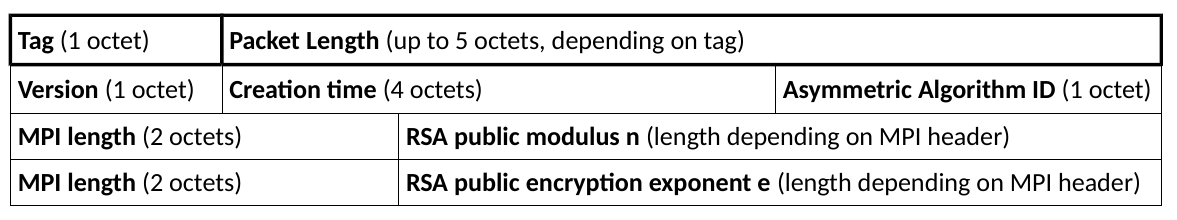
\includegraphics[width=1\linewidth]{figures/packet-key.png}
\caption[]{The structure of a key packet}
\label{fig:packet-key}
\end{figure}

Packets are composed to form the OpenPGP data structures, called transferables. This is described in section \ref{section:messageformat:transferables}. \\

\section{Transferables}
\label{section:messageformat:transferables}

In this section we give an overview of the higher-level data structures used by OpenPGP, called transferables \cite[section 11]{RFC4880}. In addition we introduce the four transferables used by OpenPGP: public key, private key, message and detached signature.  \\

Packets are representations of very basic data structures. To create OpenPGP messages and keys some of this packets are composed in a meaningful way.

A (defined) composition of packets is called transferable, since its purpose is to be transfered from one OpenPGP implementation to another or be stored and used later. \\

OpenPGP defines four different transferable types \cite[section 11]{RFC4880}: \\

First of all it is necessary to export public and secret keys in form of \textit{Transferable Public Keys} and \textit{Transferable Private Keys}. This enables storing the keys in keyrings while the OpenPGP implementation is halted. Additionally it is necessary to transmit the public key to other parties of the communication, as described in section \ref{section:openpgp:functionality}. The structure of Transferable keys is explained in section \ref{section:messageformat:keys}.  \\

The core functionality of OpenPGP is to securely transmit data. The third type of transferables therefore is a composition of packets representing such a OpenPGP Message. The structure of transferable messages is explained in section \ref{section:messageformat:messages}. \\

Furthermore it is possible to transmit signatures separated from the actual signed data, so called Detached Signatures.

\section{Keys}
\label{section:messageformat:keys}

In this section we give an overview of OpenPGP keys. We describe what an OpenPGP key-pair is and explain how multiple keys and identifying metadata are stored in one OpenPGP key. \\

An \textit{OpenPGP key} is a composition of multiple keys, identity information and other metadata, as described in  \cite[section 11.1]{RFC4880}. OpenPGP organizes key material of two kinds: \textit{primary-key} and \textit{subkeys}. The primary key is a signing key used to issue signatures of data. Furthermore the primary key is used to sign (certify) all other (critical) key parts. In addition the primary key can be used to issue certifications of other keys, as explained in chapter \ref{section:messageformat:cert}. A primary key can be used for encryption. If the primary key is only used for  signing but data encryption is still needed subkeys are required. Subkeys are additional keys inside the OpenPGP key. 

In addition to primary key and subkey, identity information is stored in the OpenPGP key in form of simple strings. The identifying information is called \textit{User ID}. Furthermore it is possible to include images, so called \textit{User Attributes}. 

Table \ref{fig:transferable-key} shows the structure of a \textit{Transferable Public Key} to illustrate this structure. \\

Because of the  asymmetric nature of OpenPGP at last one key-pair is needed for every OpenPGP secured communication. An OpenPGP key-pair consists of a Transferable Public Key and its corresponding \textit{Transferable Secret Key}. Both transferable keys contain one or more keys. 


Since the public key is shared over possibly insecure channels it needs to be protected. This is done by using the primary key to issue signatures over other key parts and appending the signatures to the key. The parts to protect are subkeys, User IDs and User Attributes. Certification is explained in section \ref{section:messageformat:cert}. \\


In addition it is possible to revoke a key or certain parts of it. This is done by signing the part and appending the signature of a certain type. It is possible to revoke a subkey, the User ID, a User Attribute or the whole OpenPGP key. Revocation is explained in section \ref{section:messageformat:cert}.

\begin{figure}[h]
	\centering
	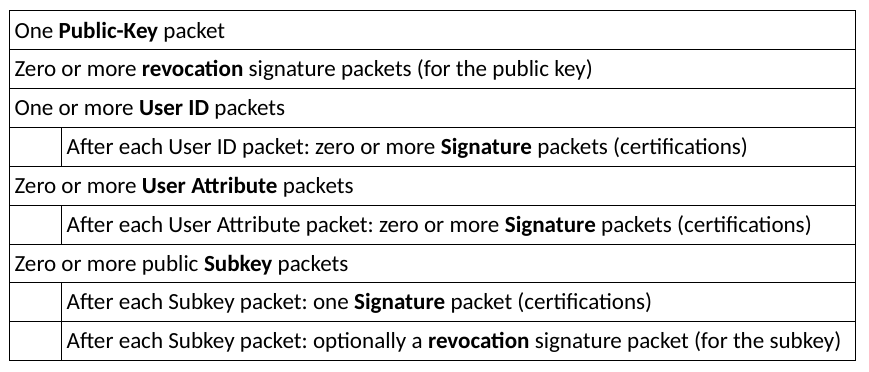
\includegraphics[width=1\linewidth]{figures/transferable-key.png}
	\caption{The structure of a Transferable Public Key}
	\label{fig:transferable-key}
\end{figure}

\section{Messages}
\label{section:messageformat:messages}

In this section we give an overview of the structure of OpenPGP messages. We explain how various packets are composed together to form an OpenPGP message. Furthermore we show how an OpenPGP transferable is constructed during encryption and decryption of an OpenPGP message. \\

An OpenPGP Message is a composition of different packets, as described in \cite[section 11.3]{RFC4880}. The actual data is contained in a \textit{Literal Data Packet}. It is possible to compress and sign the data. In addition OpenPGP provides the functionality to encrypt the data and to ensure the integrity of the encrypted data.

OpenPGP does not specify a precise structure of an \textit{OpenPGP Message}, allowing various combinations of the involved packets. For example it is not defined whether to sign the literal data and then compress or compress the data first and then sign the compressed data. In addition it is not defined whether sign-then-encrypt or encrypt-then-sign has to be performed. Thus the example shown in figure \ref{fig:transferable-msg} shows only one possibility.

\begin{figure}[h!]
	\centering
	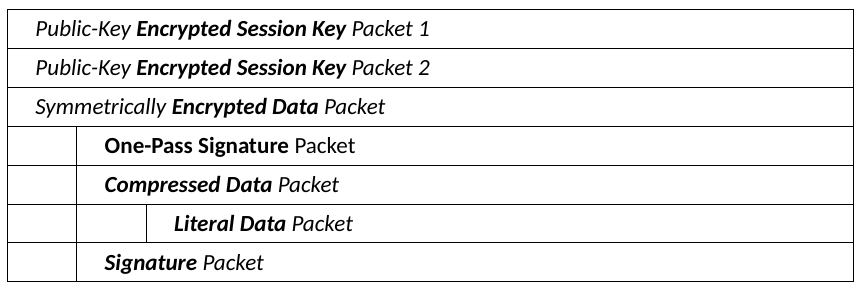
\includegraphics[width=1\linewidth]{figures/transferable-msg.png}
	\caption{The structure of a transferable OpenPGP Message}
	\label{fig:transferable-msg}
\end{figure}



\begin{figure}[h!]
	\centering
	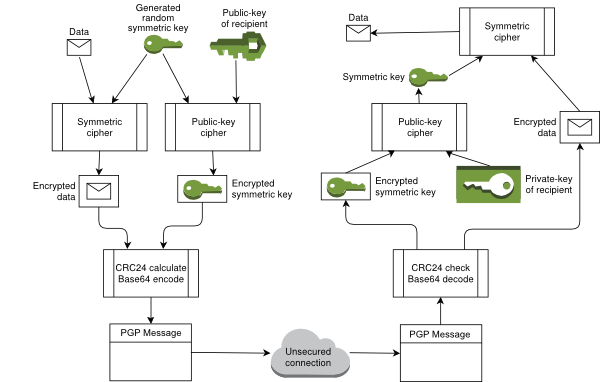
\includegraphics[width=1\linewidth]{figures/encryption}
	\caption{Visualization of process of encrypting and decrypting data}
	\label{fig:encryption}
\end{figure}


The process of encryption and decryption is shown in figure \ref{fig:encryption}. In figure \ref{fig:transferable-msg} the data is encapsulated in a \textit{Literal Data Packet}. This \textit{Literal Data Packet} is compressed, resulting in a \textit{Compressed Data Packet}. The \textit{Compressed Data Packet} is signed using the \textit{One-Pass} mechanism. The three resulting packets are encrypted using a symmetric cipher and a randomly generated session-key, resulting in a \textit{Symmetrically Encrypted Data Packet}. In this example the session-key is encrypted twice using two different public-keys, resulting in two \textit{Public-Key Encrypted Session Key Packets}. \\


To decrypt the receiver first finds the\textit{ Public-Key Encrypted Session Key Packet} encrypted using their public key and uses their private key to decrypt the session-key. Afterward the session-key is used to decrypt the three packets. The \textit{One-Pass Signature Packets} holds the information needed to calculate the hash while decompressing the \textit{Compressed Data Packet}. The resulting hash and the sender's public key are then used to verify the signature contained in the \textit{Signature Packet}. 

Afterward the \textit{Literal Data Packet} can be used. This process can be seen on the right side of figure \ref{fig:encryption}.

\section{Key Certification}
\label{section:messageformat:cert}

In this section we given an overview of how OpenPGP solves the problem of key exchange using insecure channels. We explain how the integrity of OpenPGP keys is protected. In addition we show how the binding between identity and key is ensured. Furthermore we describe how OpenPGP handles the revocation of keys. \\

OpenPGP keys are typically exchanged over an insecure channel like the Internet. During transmission all parts of the key are subject to change by an attacker. Furthermore it is possible that an attacker creates a key on their own claiming a specific identity. Therefore it is necessary to authenticate a key before using it to encrypt data or verify signatures.
This means it is required to verify the relationship between the identity information contained in an OpenPGP key and the actual identity. In addition it is required to confirm the integrity of a key. This means ensuring that no part of the key has been changed during transmission. \\

To enable this, OpenPGP uses digital signatures in two ways \cite[section 5.2.4]{RFC4880}. Self signatures are used to bind the different parts of a key together. Furthermore signatures by other keys are used to confirm the identity stored in the key, so called certifications. All signatures are formed by computing a hash-digest of the data to be signed, and then signing this hash. \\

\textbf{Binding signatures:} As shown in figure \ref{fig:transferable-key} an OpenPGP key consists of different parts. The most important parts are the primary-key, User ID  and Subkeys. To cryptographically bind those parts together signatures are used. A binding signature is formed over the packet to bind and the key to bind the packet to. Additionally some control bytes and a trailer containing metadata are appended.  \\

The following list illustrates the structure of the hashed data for a User ID binding.

\begin{itemize} \label{listing:signature}
	\item Key to bind data to:
	\begin{itemize}
		\item $0x99$ (1 octet)
		\item Length $x$ of key (2 octets)
		\item Key packet ($x$ octets)
	\end{itemize}
	
	\item Data to bind:
	\begin{itemize}
		\item $0xB4$ (1 octet)
		\item Length $y$ of User ID (4 octets)
		\item User ID packet ($y$ octets)
	\end{itemize}
	
	\item Trailer:
	\begin{itemize}
		\item Signature Version (1 octet)
		\item Signature Type (1 octet)
		\item Key Algorithm ID (1 octet)
		\item Hash-Digest Algorithm ID (1 octet)
		\item Protected subpackets ($z$ octets)
		\item Signature Version (1 octet) 
		\item $0xFF$ (1 octet)
		\item Length of trailer: 6 + $z$ (4 octets)
	\end{itemize}
\end{itemize}

To ensure the integrity of an OpenPGP key self signatures are used to bind all key parts to the primary key. This is done by signing each key part together with the primary key using the primary key. Afterward the resulting signature is appended to the key part as shown in figure \ref{fig:transferable-key}. \\

\textbf{Certification signatures} are binding signatures issued by other keys. They confirm the authenticity of the signed key part. Specifically a signature over a User ID and a key means that the issuer of the signature endorses the relation between the key, the User ID and the real identity of the entity.

The meaning of a certification is not defined by OpenPGP. More specifically it is not defined by what means the verification of the identity has to be performed. Thus it is possible that different OpenPGP users use certifications in a different way. This is further discussed in section \ref{section:concerns:usability}. \\

To verify the integrity of an OpenPGP key an implementation has to verify the respective self-signed binding signatures. 

To authenticate the identity information contained in a OpenPGP key an implementation has to verify a signature issued by an other key. For this it uses the trust model called \textit{Web of Trust}. To do so it is required to find a trust path from the own key to one of the binding signatures on the key. In addition it is necessary to verify all signatures contained in the path. The \textit{Web of Trust} is further discussed in chapter \ref{section:openpgp:functionality}. \\

Furthermore, OpenPGP provides the functionality to \textbf{revoke signatures}. This can be used to revoke parts of an OpenPGP key, for example to replace it. This is done by appending a signature of a certain type to the part to be revoked, as shown in figure \ref{fig:transferable-key}. An implementation checks if such a signature exists on the part it wants to process. The existence of such a signature invalidates the revoked part of the key. Thus the implementation is not using it. A reason for the revocation can be included into the signature's metadata. 

In general only the primary key is allowed to issue revocation signatures for its own parts. A revocation signature issued by another key does not provide any information. The only exceptions are keys who are allowed to issue revocation on the key. This is done by adding the key ID of a key to the key's metadata. An implementation checks whether the revocation signature has been issued by either the primary key or a key mentioned in the metadata. If this is not the case the revocation signature is ignored.

\section{Representation}
\label{section:messageformat:asciia}

In this section we show how OpenPGP transferables can be represented. We show how a key and a message look like while transferred. \\

Since OpenPGP defines the structure of packets as a sequence of bytes, the primary representation of a transferable is also in byte format.

For many use-cases it is sufficient to store and transmit a transferable in binary form. For example for storing the keys on a user's keyring or for transmitting over a channel which is able to transfer raw bytes. \\


Since there are channels with are not able to transfer raw bytes there is a second way to represent OpenPGP transferables. It is possible to convert a binary transferable to \myacro{ASCII}-format. Such a representation of a binary OpenPGP transferable is called \textbf{ASCII-armored} \cite[section 6]{RFC4880}.

An \myacro{ASCII}-armored OpenPGP transferable converts the raw bytes of a transferable to \myacro{ASCII} using the Base64 algorithm \citep{RFC4648}. In addition a \myacro{CRC-24} \cite[section 6.1]{RFC4880} checksum is appended to detect transmission errors. The resulting character sequence is furthermore prefixed by a header indicating the type of the transferable. Finally a footer is appended. \\

Figure \ref{fig:key} shows a sample \textit{OpenPGP Transferable Public Key}. The internal structure of this key is explained in figure \ref{fig:transferable-key}

An \myacro{ASCII}-armored OpenPGP message encrypted with the subkey contained in the \textit{Transferable Public Key} shown in figure \ref{fig:key} is shown in figure \ref{fig:msg}. The internal structure of this message is explained in figure \ref{fig:transferable-msg}. \\

\begin{figure}[p]
	\centering
	\lstinputlisting[basicstyle=\ttfamily\footnotesize]{figures/key-ecc.asc}
	\caption{Sample \myacro{ASCII}-armored transferable OpenPGP public-key}
	\label{fig:key}
\end{figure}

\begin{figure}[p]
	\centering
	\lstinputlisting[basicstyle=\ttfamily\footnotesize]{figures/msg-ecc.asc}
	\caption{Sample \myacro{ASCII}-armored transferable OpenPGP message}
	\label{fig:msg}
\end{figure}

To process the actual transferable a OpenPGP implementation first removes the header and footer. Afterward a Base64 parser is used to recover the packet bytes while calculating the \myacro{CRC-24} checksum. Finally a (optional) comparison with the appended checksum is performed.



%\section{Algorithms and Parameters}

% list algorithms from rfc, give short overview
% mention that seciruty stuff is in last chapter

% also mention IANA specification (https://www.iana.org/assignments/pgp-parameters/pgp-parameters.xhtml ?

%The OpenPGP standard allows the usage of various algorithms for encryption, integrity protection and signing. The following section lists the algorithms specified in \citep[section 9]{RFC4880}. A brief summary of those algorithm regarding their state of security and recommended key lengths is given in chapter \ref{chapter:concerns}.

%\subsection{Public-Key Algorithms}

%\subsection{Symmetric-Key Algorithms}

%\subsection{Hash Algorithms}

